% Options for packages loaded elsewhere
\PassOptionsToPackage{unicode}{hyperref}
\PassOptionsToPackage{hyphens}{url}
%
\documentclass[
]{article}
\usepackage{amsmath,amssymb}
\usepackage{lmodern}
\usepackage{iftex}
\ifPDFTeX
  \usepackage[T1]{fontenc}
  \usepackage[utf8]{inputenc}
  \usepackage{textcomp} % provide euro and other symbols
\else % if luatex or xetex
  \usepackage{unicode-math}
  \defaultfontfeatures{Scale=MatchLowercase}
  \defaultfontfeatures[\rmfamily]{Ligatures=TeX,Scale=1}
\fi
% Use upquote if available, for straight quotes in verbatim environments
\IfFileExists{upquote.sty}{\usepackage{upquote}}{}
\IfFileExists{microtype.sty}{% use microtype if available
  \usepackage[]{microtype}
  \UseMicrotypeSet[protrusion]{basicmath} % disable protrusion for tt fonts
}{}
\makeatletter
\@ifundefined{KOMAClassName}{% if non-KOMA class
  \IfFileExists{parskip.sty}{%
    \usepackage{parskip}
  }{% else
    \setlength{\parindent}{0pt}
    \setlength{\parskip}{6pt plus 2pt minus 1pt}}
}{% if KOMA class
  \KOMAoptions{parskip=half}}
\makeatother
\usepackage{xcolor}
\usepackage[margin=1in]{geometry}
\usepackage{graphicx}
\makeatletter
\def\maxwidth{\ifdim\Gin@nat@width>\linewidth\linewidth\else\Gin@nat@width\fi}
\def\maxheight{\ifdim\Gin@nat@height>\textheight\textheight\else\Gin@nat@height\fi}
\makeatother
% Scale images if necessary, so that they will not overflow the page
% margins by default, and it is still possible to overwrite the defaults
% using explicit options in \includegraphics[width, height, ...]{}
\setkeys{Gin}{width=\maxwidth,height=\maxheight,keepaspectratio}
% Set default figure placement to htbp
\makeatletter
\def\fps@figure{htbp}
\makeatother
\setlength{\emergencystretch}{3em} % prevent overfull lines
\providecommand{\tightlist}{%
  \setlength{\itemsep}{0pt}\setlength{\parskip}{0pt}}
\setcounter{secnumdepth}{5}
\newlength{\cslhangindent}
\setlength{\cslhangindent}{1.5em}
\newlength{\csllabelwidth}
\setlength{\csllabelwidth}{3em}
\newlength{\cslentryspacingunit} % times entry-spacing
\setlength{\cslentryspacingunit}{\parskip}
\newenvironment{CSLReferences}[2] % #1 hanging-ident, #2 entry spacing
 {% don't indent paragraphs
  \setlength{\parindent}{0pt}
  % turn on hanging indent if param 1 is 1
  \ifodd #1
  \let\oldpar\par
  \def\par{\hangindent=\cslhangindent\oldpar}
  \fi
  % set entry spacing
  \setlength{\parskip}{#2\cslentryspacingunit}
 }%
 {}
\usepackage{calc}
\newcommand{\CSLBlock}[1]{#1\hfill\break}
\newcommand{\CSLLeftMargin}[1]{\parbox[t]{\csllabelwidth}{#1}}
\newcommand{\CSLRightInline}[1]{\parbox[t]{\linewidth - \csllabelwidth}{#1}\break}
\newcommand{\CSLIndent}[1]{\hspace{\cslhangindent}#1}
\usepackage{setspace}
\usepackage{multicol}
\usepackage{caption}
\usepackage[italian]{babel}
\captionsetup{format=plain, font=small, labelfont=bf}
\usepackage{graphicx}
\usepackage{subcaption}
\ifLuaTeX
  \usepackage{selnolig}  % disable illegal ligatures
\fi
\IfFileExists{bookmark.sty}{\usepackage{bookmark}}{\usepackage{hyperref}}
\IfFileExists{xurl.sty}{\usepackage{xurl}}{} % add URL line breaks if available
\urlstyle{same} % disable monospaced font for URLs
\hypersetup{
  pdftitle={Plant Growth},
  pdfauthor={Elisa Mancinelli},
  hidelinks,
  pdfcreator={LaTeX via pandoc}}

\title{Plant Growth}
\author{Elisa Mancinelli}
\date{2023-03-09}

\begin{document}
\maketitle

\pagenumbering{gobble}

%\begin{titlepage}
	\begin{center}
		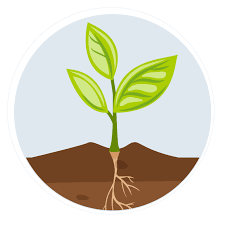
\includegraphics[width=0.25\linewidth]{logo/PlantLogo.png}
	\end{center}
	
	\begin{center}
		\begin{Large}
			\textbf{Università di Padova}
			
			Dipartimento di Psicologia dello Sviluppo e della Socializzazione
		\end{Large}
		
	\end{center}
	
	\vspace{3mm}
	\begin{center}
		\begin{large}
			Ph.D. Course in Brain Mind and Computer Science (XXXVII Cycle)
		\end{large}
		
		\begin{huge}
			\bfseries
			Plant Growth: Crescita delle piante in base a tre condizioni sperimentali
		\end{huge}
		
		
	\end{center}
	
	\vspace{2cm}
	\begin{multicols}{2}
		\begin{flushleft}
%			\begin{large}
				\textbf{Advisor:} Prof. Pinco Pallino
				
				\textbf{Co-Advisor:} Prof. Pallino Pinco
	%		\end{large}
			
		\end{flushleft}
		\columnbreak
		\begin{flushright}
			\vspace{1.5cm}
			
				\textbf{Ph.D. Candidate:} Elisa Mancinelli 
			
		\end{flushright}
		
	\end{multicols}

\vspace{2cm}
	
	\begin{center}
		Academic Year: 2023/2024
	\end{center}
	
	

\hypersetup{linkcolor = black}
\newpage
\renewcommand{\contentsname}{Indice}
\pagenumbering{roman}
\tableofcontents
\addcontentsline{toc}{section}{\contentsname}

\newpage

% list of figures have to be added manually to table of contents
\listoffigures % Per toogliere la lista delle figura, aggiungere % all'inizio della riga

\newpage
\listoftables % Per toogliere la lista delle tabelle, aggiungere % all'inizio della riga

\doublespacing

\newpage
\pagenumbering{arabic}
\hypersetup{linkcolor = blue}

{
\setcounter{tocdepth}{2}
\tableofcontents
}
\hypertarget{introduzione}{%
\section{Introduzione}\label{introduzione}}

Bello studiar le piante

Citare articolo 1 (Epifania, Anselmi, and Robusto 2020) e poi il secondo
articolo (Bianchi, Anselmi, and Robusto 2020)

\hypertarget{metodo}{%
\section{Metodo}\label{metodo}}

Le condizioni con sui studiamo le piante

\begin{itemize}
\tightlist
\item
  Una condizione di controllo
\item
  Due condizioni sperimentali
\end{itemize}

\hypertarget{risultati}{%
\section{Risultati}\label{risultati}}

\begin{itemize}
\tightlist
\item
  Inserite una Figura con tre sottofigure (due foto e il grafico del
  vostro dataset) con rispettive cross-reference nel testo
\end{itemize}

Nella figura \ref{fig:elef} troviamo un mega elefante

\begin{figure}
\centering
\caption{Elefante.}
\label{fig:elef}

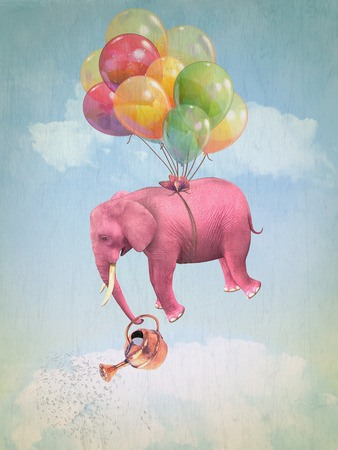
\includegraphics[width=0.5\linewidth]{image/elefante} 

\end{figure}

Nella Figura \ref{fig:figTripla} si trovano due immagini a caso e il
grafico delle piante.

Nello specifico, in Figura \ref{sub:elefant} c'è un elefante, mentre in
Figura \ref{sub:testa} c'è una mega testa colorata.Invece, in Figura
\ref{sub:grafico} c'è un plot del dataset Plant growth

\begin{figure}
  \centering
  \begin{subfigure}{0.3\textwidth}

\begin{center}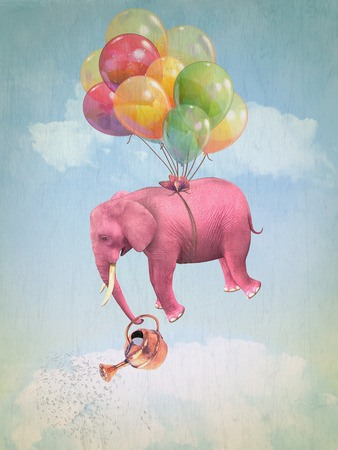
\includegraphics[width=0.8\linewidth]{image/elefante} \end{center}

\caption{Elefante.}
\label{sub:elefant}
\end{subfigure}
\begin{subfigure}{0.3\textwidth}

\begin{center}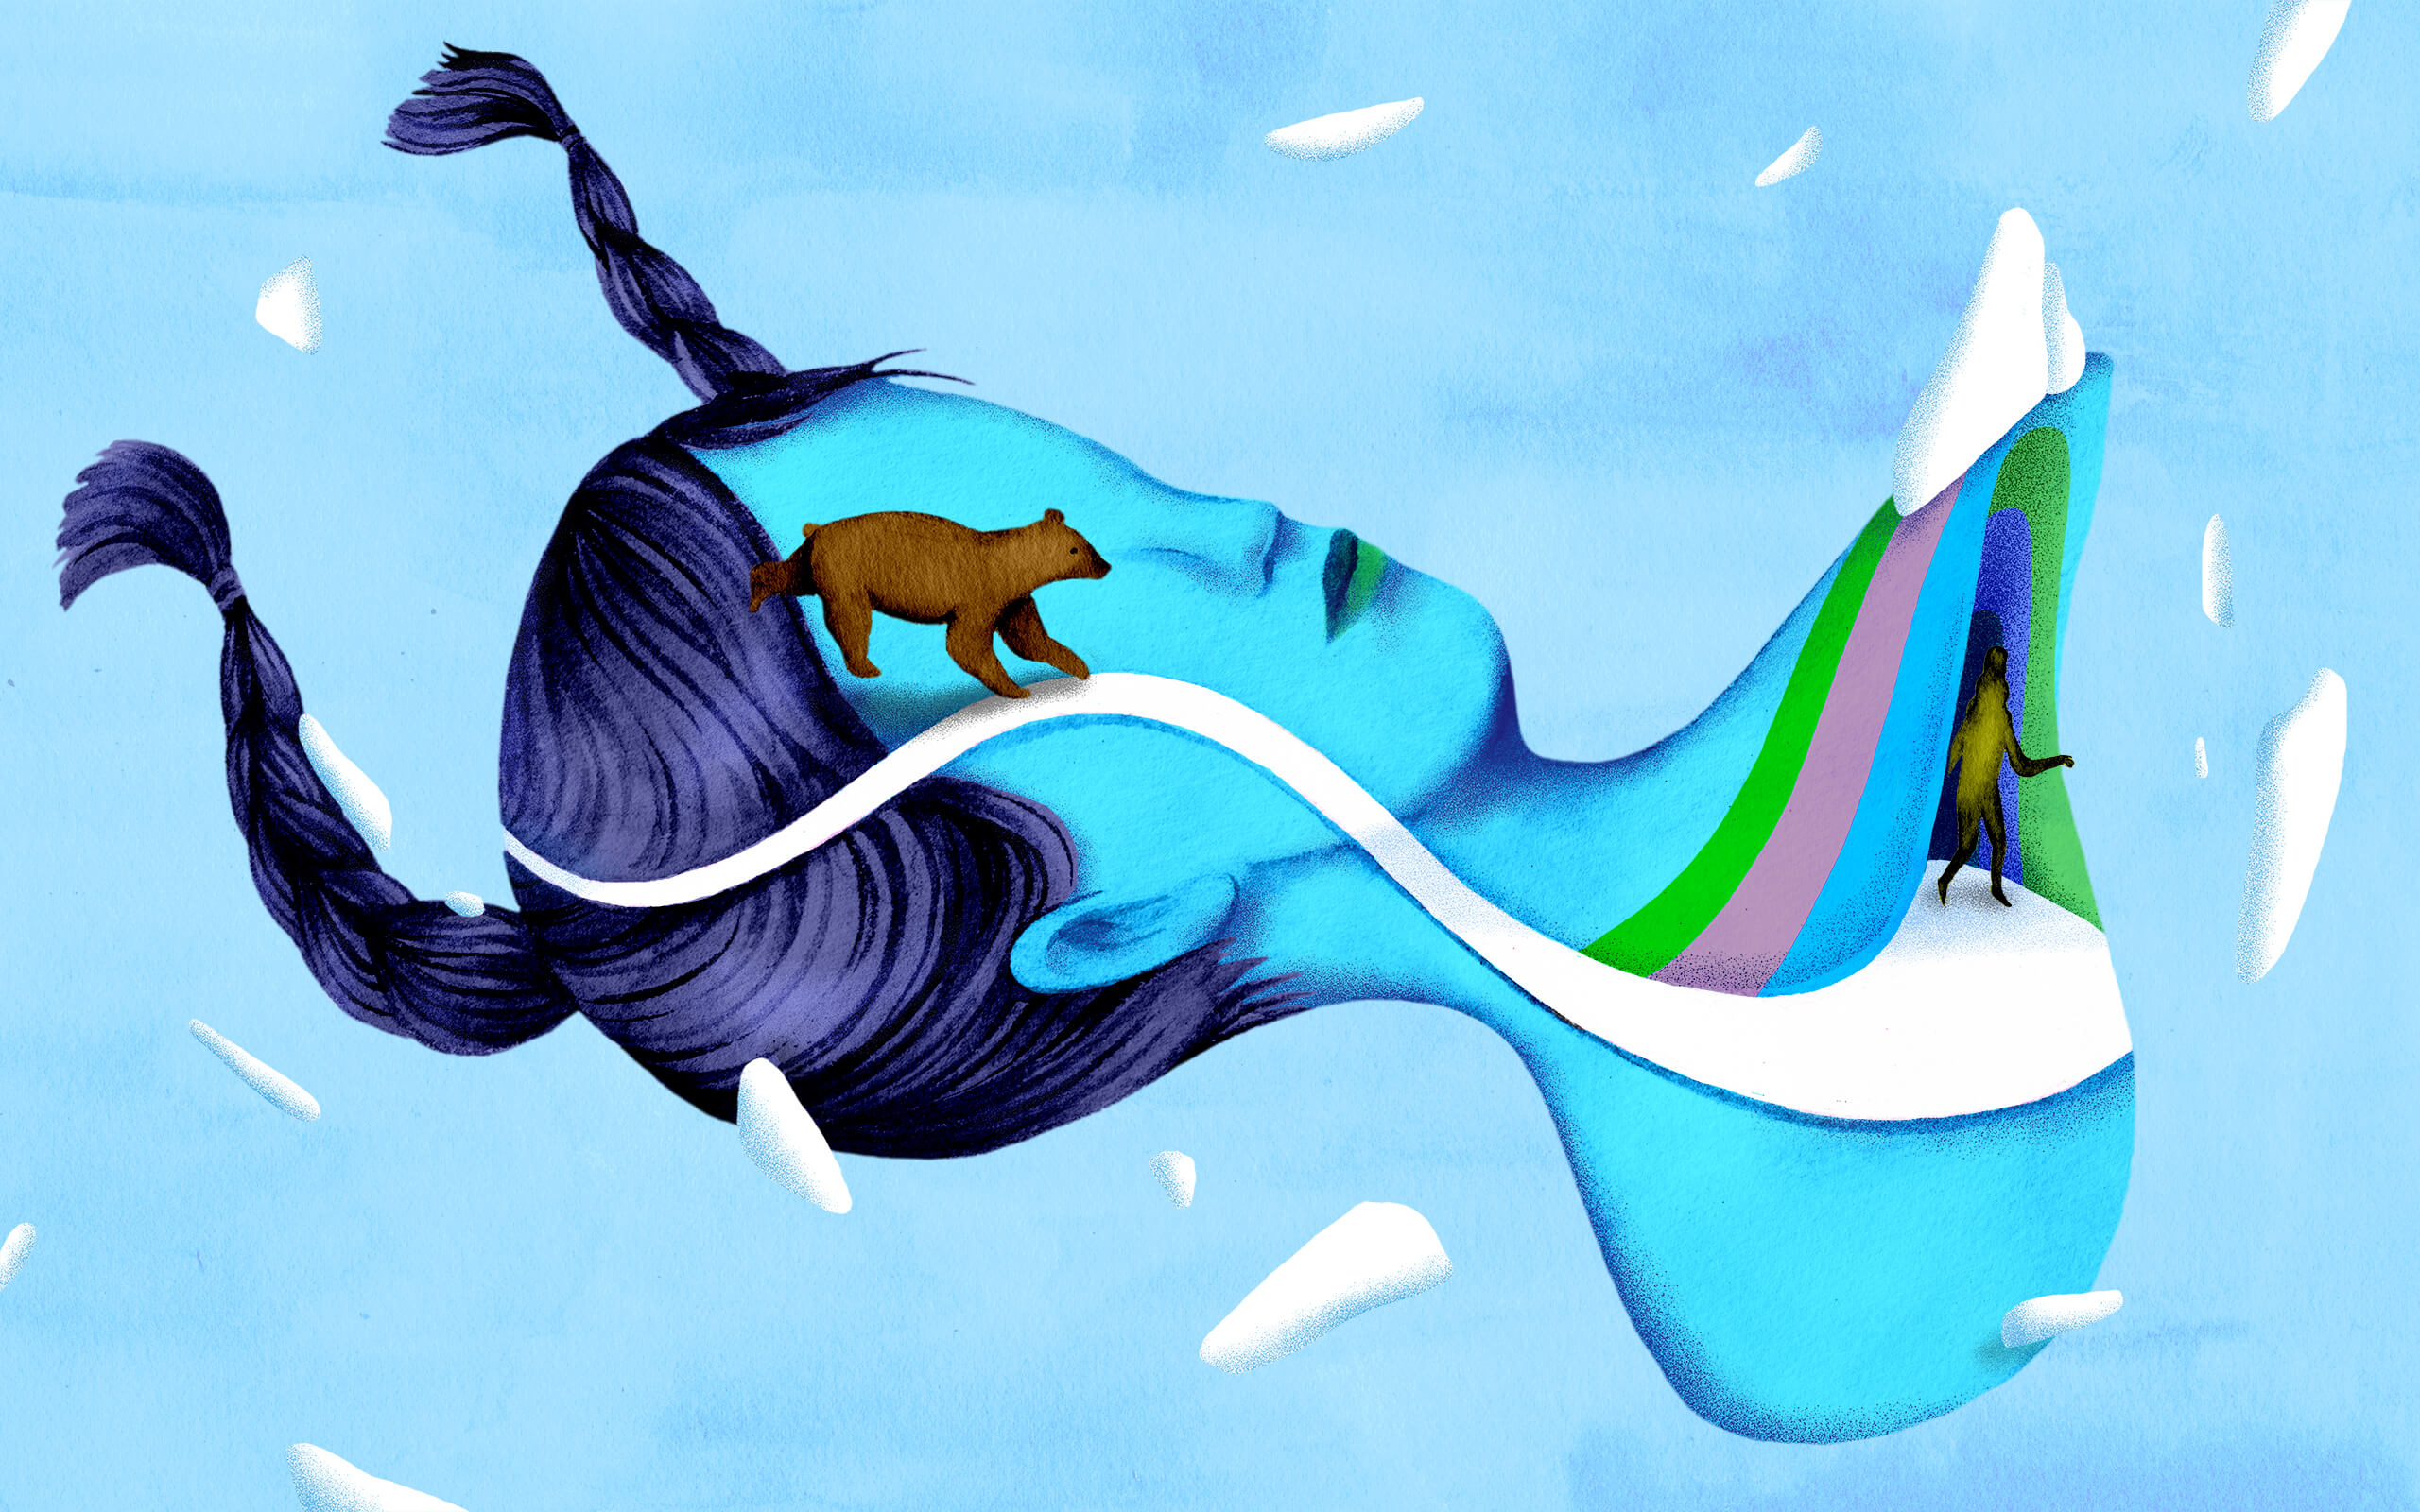
\includegraphics[width=0.8\linewidth]{image/daydreaming5final} \end{center}

\caption{Testa colorata}
\label{sub:testa}
\end{subfigure}
\begin{subfigure}{0.3\textwidth}

\begin{center}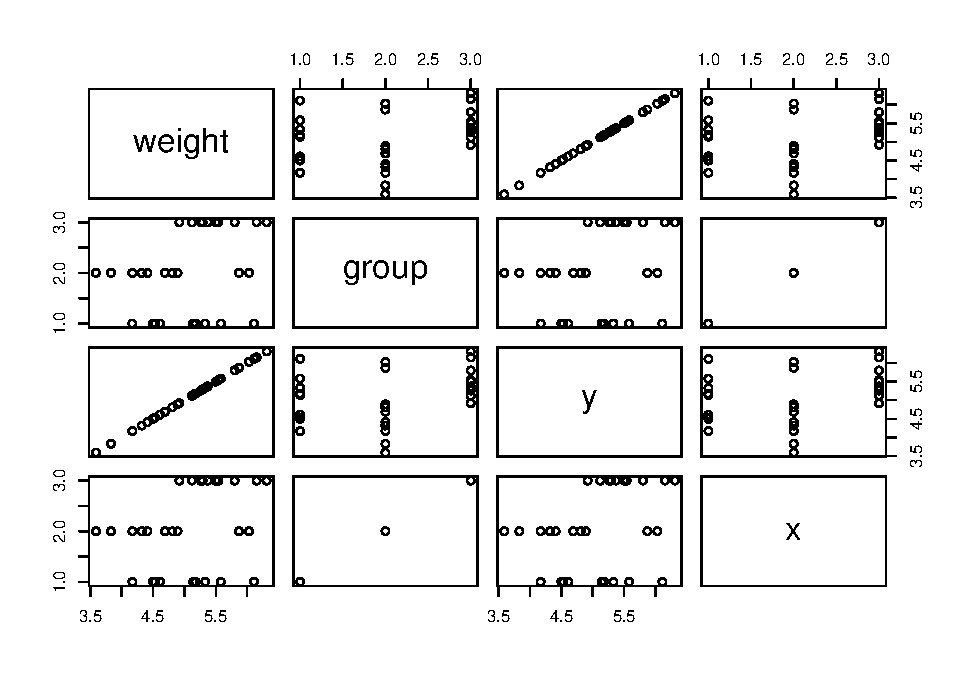
\includegraphics[width=0.8\linewidth]{Latex_knits_09-03-23_files/figure-latex/unnamed-chunk-4-1} \end{center}

\caption{Grafico Piante.}
\label{sub:grafico}
\end{subfigure}
\caption{Figura Tripla}
\label{fig:figTripla}
\end{figure}

I risultati della Figura \ref{sub:grafico} sono anche riprotati nella
Tabella \ref{tab:tabPiante}

\begin{table}[ht]
\centering
\caption{Tabella Plant Growth} 
\label{tab:tabPiante}
\begin{tabular}{rrlrl}
  \hline
 & weight & group & y & x \\ 
  \hline
1 & 4.17 & ctrl & 4.17 & ctrl \\ 
  2 & 5.58 & ctrl & 5.58 & ctrl \\ 
  3 & 5.18 & ctrl & 5.18 & ctrl \\ 
  4 & 6.11 & ctrl & 6.11 & ctrl \\ 
  5 & 4.50 & ctrl & 4.50 & ctrl \\ 
  6 & 4.61 & ctrl & 4.61 & ctrl \\ 
  7 & 5.17 & ctrl & 5.17 & ctrl \\ 
  8 & 4.53 & ctrl & 4.53 & ctrl \\ 
  9 & 5.33 & ctrl & 5.33 & ctrl \\ 
  10 & 5.14 & ctrl & 5.14 & ctrl \\ 
   \hline
\end{tabular}
\end{table}

\clearpage

\hypertarget{bibliografia}{%
\section*{Bibliografia}\label{bibliografia}}
\addcontentsline{toc}{section}{Bibliografia}

\hypertarget{refs}{}
\begin{CSLReferences}{1}{0}
\leavevmode\vadjust pre{\hypertarget{ref-epifania2020implicit}{}}%
Bianchi, Ottavia M, Pasquale Anselmi, and Egidio Robusto. 2020.
{``Implicit Measures with Reproducible Results: The implicitMeasures
Package.''} \emph{Journal of Open Source Software} 5 (52): 2394.
\url{https://doi.org/https:/doi.org/10.21105/joss.02394}.

\leavevmode\vadjust pre{\hypertarget{ref-epifania2020dscoreapp}{}}%
Epifania, Ottavia M, Pasquale Anselmi, and Egidio Robusto. 2020.
{``DscoreApp: A Shiny Web Application for the Computation of the
Implicit Association Test d-Score.''} \emph{Frontiers in Psychology} 10:
2938. \url{https://doi.org/https:/doi.org/10.3389/fpsyg.2019.02938}.

\end{CSLReferences}

\end{document}
